% Exercise ID: MAT_A12OTIMI_ESTU_MRE_004
% Module: Módulo A12 - Otimização | Concept: Estudo da Monotonia
% Type: monotonia_real | Difficulty: 2/5
% Tags: monotonia, gráfico, contexto_real, velocidade, valor_absoluto, constante
% Author: Professor | Date: 2025-11-26

\exercicio{
Um ciclista inicia um percurso às 9h00. Nos primeiros 2 km, a sua velocidade varia de acordo com $v(x) = |x-1|$ (em km/h), onde $x$ é a distância percorrida em km. Depois, mantém uma velocidade constante de 1 km/h até aos 3 km. O gráfico mostra a evolução da velocidade ao longo do percurso.

\begin{center}
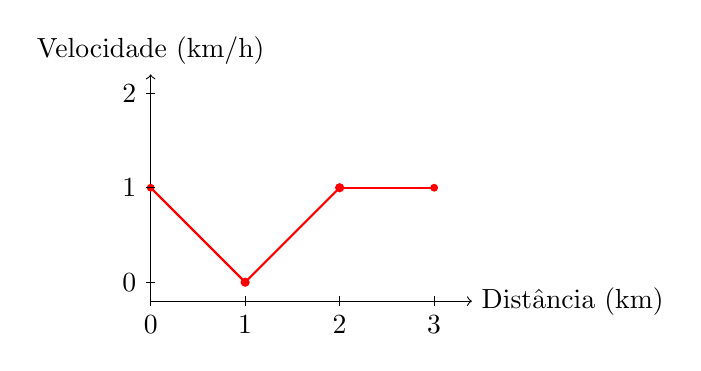
\begin{tikzpicture}[scale=1.2]
  \draw[->] (0,0) -- (3.4,0) node[right] {Distância (km)};
  \draw[->] (0,0) -- (0,2.4) node[above] {Velocidade (km/h)};
  % ramos
  \draw[thick, red, domain=0:2, samples=50] plot (\x, {abs(\x-1)+0.2});
  \draw[thick, red] (2,1.2) -- (3,1.2);
  % pontos
  \filldraw[red] (0,1.2) circle (1pt);
  \filldraw[red] (1,0.2) circle (1.2pt);
  \filldraw[red] (2,1.2) circle (1.2pt);
  \filldraw[red] (3,1.2) circle (1pt);
  % marcas x
  \foreach \x in {0,1,2,3} \draw (\x,0.05) -- (\x,-0.05) node[below] {\x};
  % marcas y
  \foreach \y in {0,1,2} \draw (0.05,\y+0.2) -- (-0.05,\y+0.2) node[left] {\y};
\end{tikzpicture}
\end{center}
}

\subexercicio{Durante que intervalo de distância a velocidade esteve a aumentar?}

\subexercicio{Durante que intervalo de distância a velocidade esteve a diminuir?}

\subexercicio{Qual foi a velocidade mínima atingida e em que ponto do percurso isso aconteceu?}

\subexercicio{Interpreta o significado dos diferentes ramos do gráfico no contexto do percurso do ciclista.}
